\subsection{Pole placement}\label{chapter_PolePlace}

The pole placement is the most important step in developing a state space controller. With a state space controller it is possible - if the process is controllable - to move the existing poles of the given process, like figure \ref{fig:simpleProcess} shows, to a specific position in the closed loop (figure \ref{fig:simpleProcess_Controller}). There are several possibilities to arrange the poles in the s-plane to gain a short rise time, a short control settling time and no ringing. The more the poles are moved to the negative real axes, the faster the closed loop process will be. But for that, very high actuating variables are needed, that might not be available. For the quadrocopter, the motors are the limiting factor.

As mentioned in chapter \ref{chapter_StateSpace}, the example process is controllable, so the poles can be placed. 
The poles of the process are at [-1 -1 -1] in the s-plane and the corresponding step response is:

\begin{figure}
	\centering
		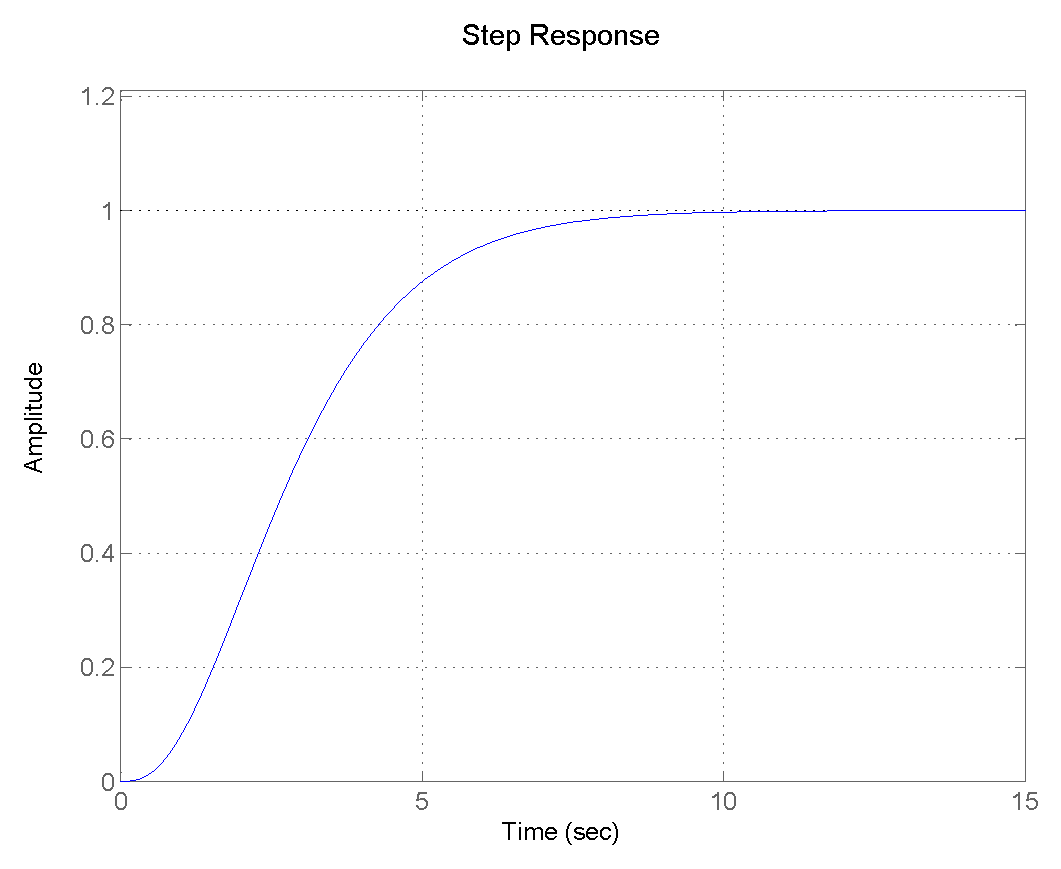
\includegraphics[width=0.70\textwidth]{03_Grafiken/step_Process.pdf}
	\caption{Step response of the process without the state space controller}
	\label{fig:stepProcess}
\end{figure}

This is not a good result, although the poles are on the left side of the s-plane. To make the step response faster in the closed loop, the poles are moved to [-4 -3 -2]. These new positions, the poles are moved to, are chosen without any ulterior motive.

So how to calculate the state variable feedback factors \textit{KRx}?
The process can be described in a very nice vector notation, including the state space matrices. The D matrix is zero in this process. The uvec in the gain blocks in figure \ref{fig:simpleProcess_Vector} shows, that the output is a vector and not a single value as in the 'normal' block diagrams.

\begin{figure}
	\centering
		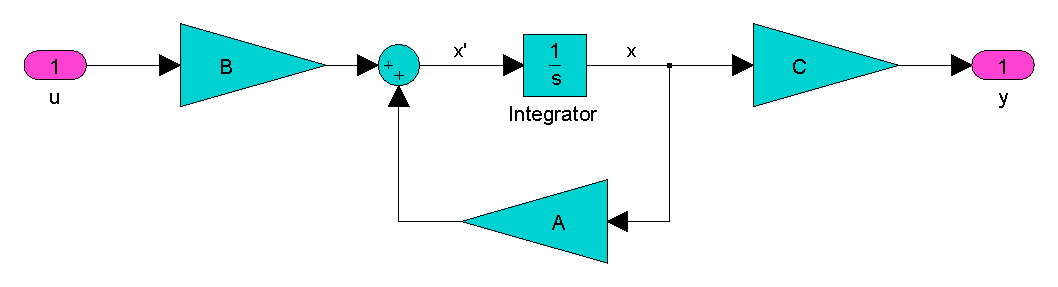
\includegraphics[width=1.00\textwidth]{03_Grafiken/simpleProcess_Vector.pdf}
	\caption{Matrix view of the process}
	\label{fig:simpleProcess_Vector}
\end{figure}

\begin{align}
	\underline{x}' & = \underline{A} * \underline{x} + \underline{B} * u \\
	y  & = \underline{C} * \underline{x}
\end{align}

The target of the pole placement is, to transform this open loop process into a closed loop control with the desired poles.

\begin{figure}
	\centering
		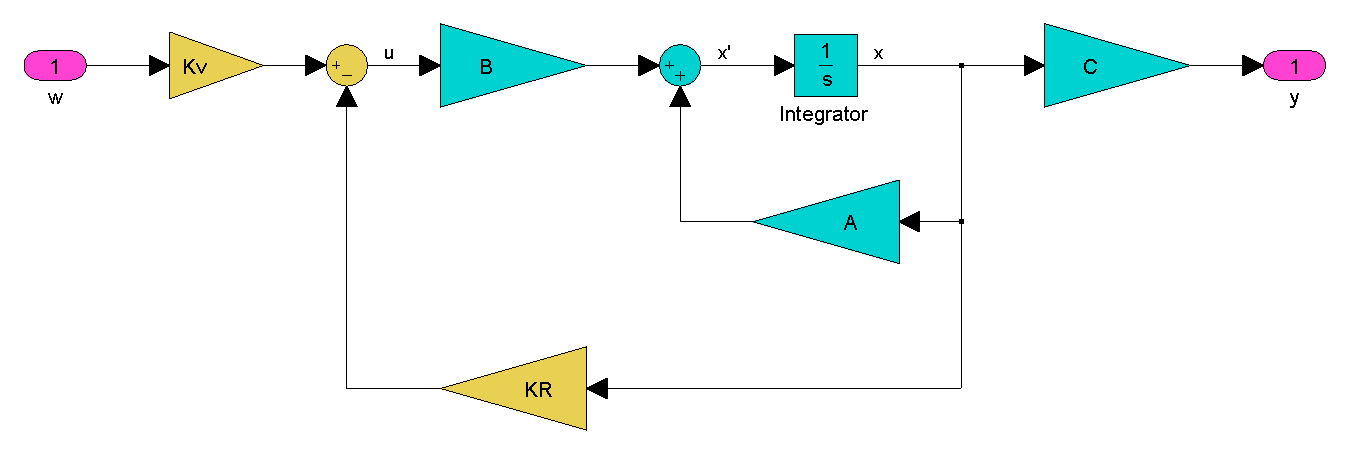
\includegraphics[width=1.00\textwidth]{03_Grafiken/simpleProcess_VectorControl.pdf}
	\caption{Matrix view of the process including the state space controller}
	\label{fig:simpleProcess_VectorControl}
\end{figure}

Therefore the input \textit{u} (in front of the 'B gain block') can be described:
\begin{align}
	u ~=~ Kv*w - \underline{KR}*\underline{x} 
\end{align}

Finally the closed loop control equations are:
\begin{align}
	\underline{x}' & = (\underline{A} - \underline{B} * \underline{KR}) * \underline{x} + \underline{B} * Kv * u \\
	y  & = \underline{C} * \underline{x}
\end{align}

And the new system matrix for the closed loop is:
\begin{align}
	\underline{A_{CL}} ~=~ \underline{A} - \underline{B} *\underline{KR} 
\end{align}

With this 'formula' it is easy to calculate the state variable feedback factors \textit{KRx} if the state matrix of the open loop and the state matrix of the desired closed loop is known. 
So, for this example - recognizing that the poles are moved to [-4 -3 -2] - the \textit{KR} factors are [6 11 6]. The step response of the closed loop seems to be much faster:

\begin{figure}
	\centering
		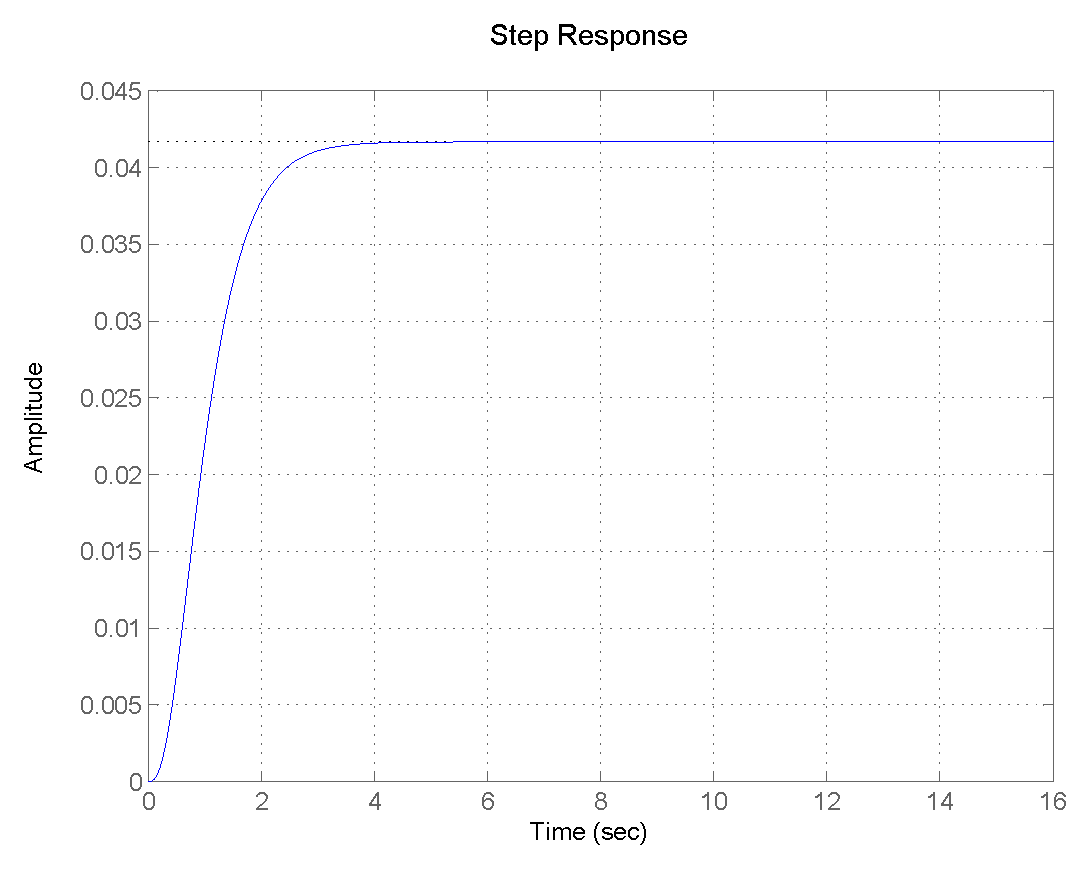
\includegraphics[width=0.7\textwidth]{03_Grafiken/step_Controller_withoutKV.pdf}
	\caption{Step response of the process including the state space controller with a pre-intensification equal one}
	\label{fig:stepControlKV1}
\end{figure}

The step response is much faster - but - it only steps to $y_\infty = 0.0417$. The second part of the state space controller has to be calculated. To calculate the pre-intensification factor \textit{Kv} for a very easy SISO system, the steady state value of the system's input must be divided by the system's output \myeqref{Kveasy}. 
\begin{align}\label{Kveasy}
	Kv = \frac{u}{y_\infty}
\end{align}

For the system of the quadrocopter which is a MIMO system, the calculation of the pre-intensification factor \textit{Kv} is much more complex \myeqref{Kvcomplex}.
\begin{align}\label{Kvcomplex}
	Kv = -\left[\underline{C} * (\underline{A} - \underline{B} * \underline{KR})^{-1} * \underline{B} \right]^{-1}
\end{align}

The example used here is a simple system and the pre-intensification factor \textit{Kv} can be calculated easily:
\begin{align}
	Kv = \frac{1}{0.0417} \approx 24
\end{align}

With this pre-intensification factor the step response really steps up to one:

\begin{figure}
	\centering
		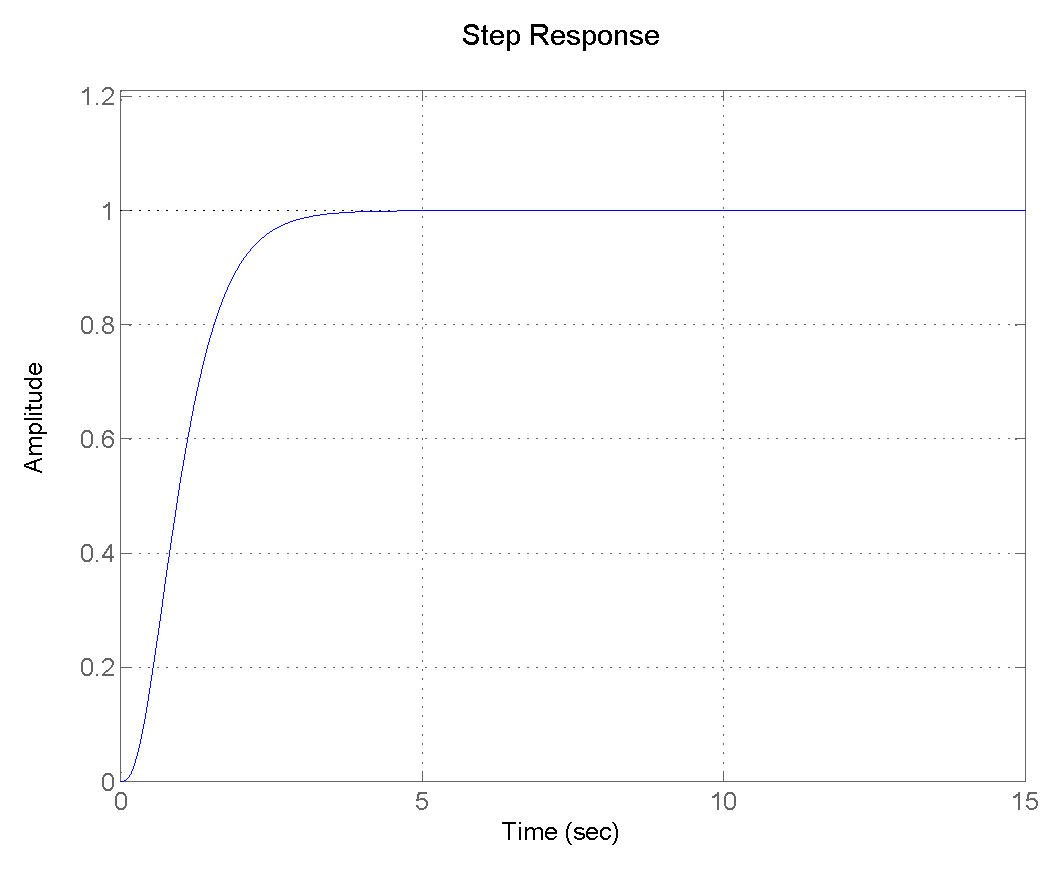
\includegraphics[width=0.70\textwidth]{03_Grafiken/step_Controller_withKV.pdf}
	\caption{Step response of the process including the state space controller and a calculated pre-intensification}
	\label{fig:stepControlKV24}
\end{figure}
